The experiments use CartPole-v1 from Gymnasium~\cite{towers2024gymnasium}. The observation space has 4
continuous variables (cart position, cart velocity, pole angle, pole angular
velocity) and the action space has 2 discrete actions (push left, push right).
Episodes terminate when the pole angle exceeds $\pm 12^\circ$, the cart position
exceeds $\pm 2.4$, or 500 steps are reached. The reward is $+1$ per step,
making the maximum episode return 500.

\begin{figure}[t]
  \centering
  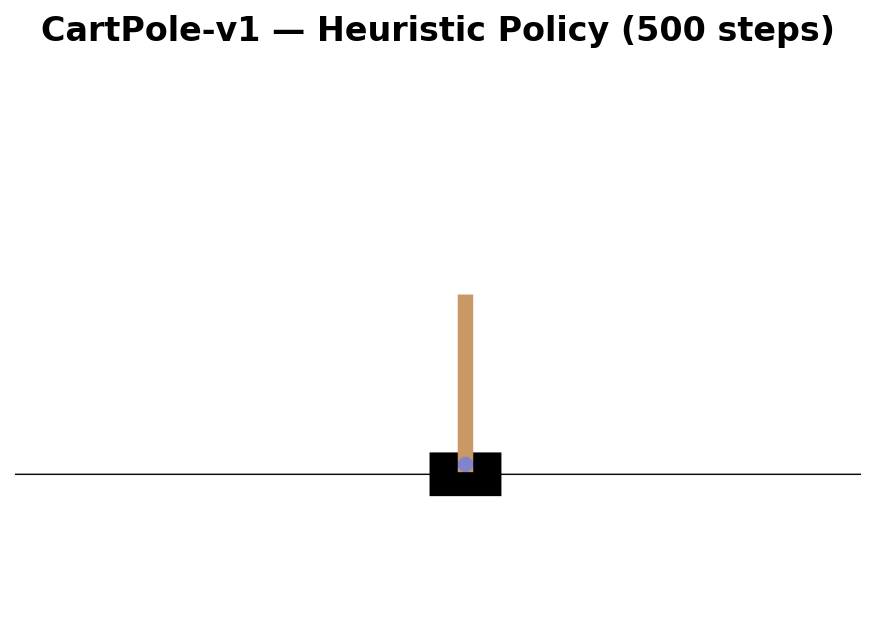
\includegraphics[width=0.85\linewidth]{../outputs/figures/cartpole_screenshot.png}
  \caption{CartPole-v1 environment. The goal is to balance the pole by moving the cart. The heuristic policy (shown) achieves the maximum 500-step return.}
  \label{fig:cartpole}
\end{figure}

Both agents use the hyperparameters listed in Table~\ref{tab:hparams}.

\begin{table}[t]
  \centering
  \caption{Shared DQN hyperparameters for all configurations.}
  \label{tab:hparams}
  \footnotesize
  \begin{tabular}{lr}
    \hline
    Hyperparameter & Value \\
    \hline
    Discount factor ($\gamma$) & 0.99 \\
    Learning rate & 0.001 \\
    Optimizer & Adam \\
    Batch size & 16 \\
    Replay buffer size & 50,000 \\
    Target update interval & 100 steps \\
    Learning starts & 16 steps \\
    Epsilon start & 1.0 \\
    Epsilon end & 0.05 \\
    Gradient clipping norm & 10.0 \\
    Loss function & Smooth L1 (Huber) \\
    Greedy evaluation episodes & 20 \\
    Log interval & 10 episodes \\
    \hline
  \end{tabular}
\end{table}

We evaluate eight main configurations, summarized in Table~\ref{tab:configs}.

\begin{table}[t]
  \centering
  \caption{Experimental configurations. MLP-L1 uses 3 hidden units (23 params). VQC-L1 uses 1 layer (22 params). VQC-L3 uses 3 layers (46 params). Dueling variants add value/advantage split; Double variants add Double DQN.}
  \label{tab:configs}
  \footnotesize
  \begin{tabular}{lccc}
    \hline
    Configuration & Agent & Episodes & $\epsilon$ decay \\
    \hline
    Standard (5 seeds) & MLP-L1 / VQC-L1 & 100 & 2000 steps \\
    Dueling (3 seeds) & MLP-L1 / VQC-L1 & 100 & 800 steps \\
    Double-Dueling (3 seeds) & MLP-L1 / VQC-L1 & 100 & 800 steps \\
    Extended (3 seeds) & MLP-L1 / VQC-L1 & 500 & 4000 steps \\
    \hline
  \end{tabular}
\end{table}

All configurations use 5 seeds ($0, 1, 2, 4, 7$) for the main 100-episode
comparisons and 3 seeds for the extended 500-episode runs. The 100-episode
configurations use $\epsilon$ decay over 2000 environment steps; the extended
500-episode runs use decay over 4000 steps. The Double DQN and Dueling DQN
variants use 3 seeds with $\epsilon$ decay over 800 steps.

The classical MLP was executed with PyTorch on an NVIDIA GeForce RTX 5090 (GPU).
The VQC was simulated with PennyLane~\cite{bergholm2018pennylane} \texttt{default.qubit} backend on CPU. The
timing comparison therefore conflates GPU-vs-CPU and PyTorch-vs-simulator
overheads; reported VQC time multipliers should be interpreted as upper bounds
on the simulation cost. The software stack used PyTorch 2.12.0+cu130,
Gymnasium 1.3.0, and PennyLane 0.45.0.

The distillation experiments use the same model architectures trained with
cross-entropy loss over 20 epochs with 512 sampled states (or 50 epochs with
1024 samples for the MLP raw distill run, as noted in Table~\ref{tab:fuzzy-distill}).
The fuzzy teacher heuristic is $a = \mathbf{1}[\theta + 0.25\dot{\theta}
+ 0.01x + 0.01\dot{x} > 0]$, which achieves 500.00 reward as a policy but is
used here only as a labeling source.

The reported metrics are reward per episode, final mean reward over the last 20
training episodes (or last 10 for extended runs), greedy evaluation reward over
20 episodes, trainable parameter count, and wall-clock training time. Random
($a_t \sim \text{Uniform}(\mathcal{A})$) and heuristic (the same fuzzy rule used
as the teacher) policies are included as non-learning reference baselines.

The complete codebase is organized as a Python package under \texttt{src/qrl/}
with modules for agents (replay buffer), environments (preprocessing), models
(MLP, VQC, factory), training (DQN loop, experiment runner), and utilities
(seeding, parameter counting). Experiments are configured via YAML files and
executed through \texttt{scripts/train.py} with CLI overrides for rapid
exploration. All figures and tables are reproducible from the YAML configs and
output CSV/JSON artifacts. The test suite comprises 24 tests covering model
forward passes, preprocessing, replay buffer, epsilon scheduling, fuzzy actions,
and dueling architectures.
